% \section{PROPOSED METHOD}
% \label{sec:proposed_method}

% \subsection{System Overview}
% The proposed federated multi-task framework employs a hierarchical architecture designed for real-time NLU applications. As illustrated in Fig.~\ref{fig:framework_pipeline}, the system consists of a central orchestration server and multiple heterogeneous client nodes. The central server maintains the global state through a Parameter Server and manages the Model Aggregation logic. Communication is established via low-latency WebSockets, facilitating bidirectional exchange of model updates and aggregated parameters.

% \begin{figure*}[t]
%     \centering
%     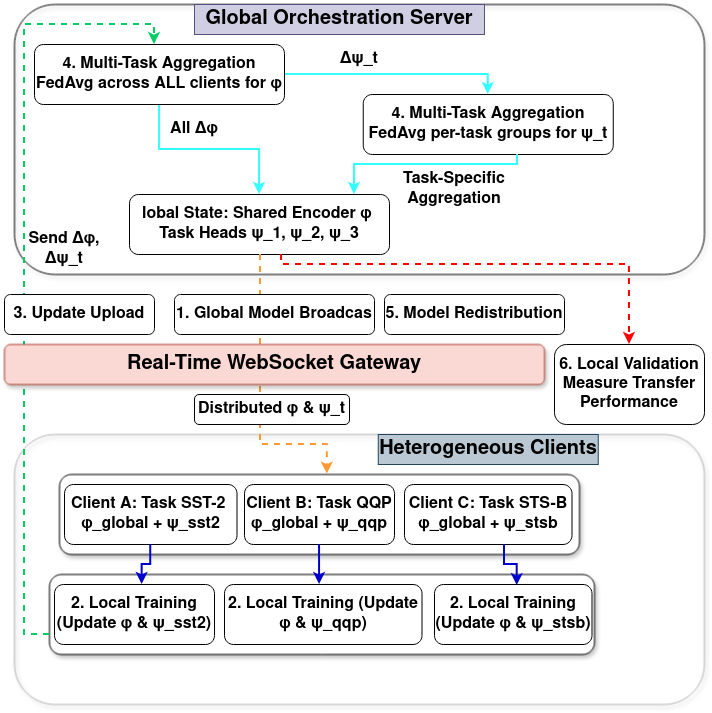
\includegraphics[width=1.0\textwidth]{plots/FL_MTL_FRAME_WORK.png}
%     \caption{Architecture of the Proposed Real-time Federated Multi-Task Learning Framework. The system enables seamless integration of streaming data processing and collaborative model refinement.}
%     \label{fig:framework_pipeline}
% \end{figure*}

% Federated system components and privacy constraints consists of:
% \begin{itemize}
%     \item \textbf{Global server} $\mathcal{S}$: coordinates client sampling, model broadcast, and aggregation.
%     \item \textbf{Distributed clients} $\mathcal{C}$: edge devices/silos that keep raw text data local.
%     \item \textbf{Task set} $\mathcal{K}$: heterogeneous NLU tasks (e.g., intent classification, sentiment analysis, sequence labeling).
%     \item \textbf{Local datasets} $\mathcal{D}_c^t$: private, time-indexed data available at client $c$ at round $t$.
% \end{itemize}

% For privacy, raw samples are never uploaded. Each client transmits only model updates (or compressed adapter/head updates), and aggregation is performed on the server side \cite{mcmahan2017fedavg,elbakary2025mira}. This aligns with the standard federated privacy model in which data locality is preserved while collaborative training is enabled.


% \subsection{Small Language Model Backbone}
% The framework utilizes specialized Small Language Models (SLMs) to balance computational efficiency and linguistic performance. Our current implementation supports DistilBERT \cite{sanh2019distilbert}, BERT-Medium \cite{devlin2018bert}, and MiniLM \cite{wang2020minilm} architectures. These models serve as the shared feature extractor (encoder), which is fine-tuned collaboratively across the federated network. By using SLMs, we achieve a significant reduction in communication overhead compared to standard-sized transformers.

% \subsection{Multi-Task Learning Strategy}
% We adopt a hybrid parameter-sharing strategy. The lower transformer layers (encoder) are shared across all tasks to capture universal linguistic representations. In contrast, the upper layers consist of task-specific classification or regression heads. To mitigate negative transfer, we implement an adaptive loss weighting mechanism:
% \begin{equation}
%     \mathcal{L}_{total} = \sum_{j=1}^{T} \alpha_j \mathcal{L}_j
% \end{equation}
% where $\alpha_j$ is dynamically adjusted based on the convergence rate of each task $j$.

% We parameterize shared encoder and task-specific heads by
% \begin{equation}
% \Theta = \{\theta_e, \{\theta_k\}_{k=1}^{K}\},
% \end{equation}
% where $\theta_e$ is a shared small-language-model encoder and $\theta_k$ is the task-specific prediction head for task $k$ \cite{chen2024fedbone,zhou2025mfed,elbakary2025mira}.

% For an input-output pair $(x,y)$ from task $k$, prediction is
% \begin{equation}
% \hat{y} = h_k\big(f_e(x;\theta_e);\theta_k\big),
% \end{equation}
% where $f_e(\cdot)$ denotes the shared encoder and $h_k(\cdot)$ denotes the task head. This design supports parameter sharing for transferable linguistic features while retaining task-level specialization.

% \subsection{Federated Optimization and Real-time Adaptation}
% The federated optimization process is detailed in Algorithm~\ref{alg:rt_fmtl}. The system facilitates real-time adaptation by allowing clients to synchronize updates asynchronously via WebSockets. The server aggregates updates using a task-aware variant of FedAvg, ensuring that noisy updates from heterogeneous data sources (Non-IID) are properly regularized.

% \begin{algorithm}
% \caption{Real-Time Federated Multi-Task Learning (RT-FMTL)}
% \label{alg:rt_fmtl}
% \begin{algorithmic}[1]
% \STATE \textbf{Server Initialize:} Shared core $\phi_0$, Task heads $\{\psi_{j,0}\}_{j=1}^T$
% \FOR{each round $t = 1, 2, \dots$}
%     \STATE Server broadcasts $\phi_t, \psi_{Task(k),t}$ to client $k \in K$ via WebSockets
%     \FOR{each client $k \in K$ \textbf{in parallel}}
%         \STATE Local training: $\{\Delta\phi_k, \Delta\psi_{Task(k),k}\} \leftarrow \text{LocalUpdate}(\mathcal{D}_k, \phi_t, \psi_{Task(k),t})$
%         \STATE Send updates $\{\Delta\phi_k, \Delta\psi_{Task(k),k}\}$ to Server via WebSockets
%     \ENDFOR
%     \STATE \textbf{Task-Aware Aggregation:}
%     \STATE \quad $\phi_{t+1} \leftarrow \phi_t + \eta \sum_{k=1}^K \frac{n_k}{N} \Delta\phi_k$ \COMMENT{Universal Knowledge}
%     \FOR{each task $j \in \{1,\dots,T\}$ \textbf{in parallel}}
%         \STATE $\psi_{j,t+1} \leftarrow \psi_{j,t} + \eta \sum_{k \in K_j} \frac{n_k}{N_j} \Delta\psi_{j,k}$ \COMMENT{Heads Specialization}
%     \ENDFOR
%     \STATE Server redistributes $\{\phi_{t+1}, \psi_{Task(k),t+1}\}$ for Local Validation
% \ENDFOR
% \end{algorithmic}
% \end{algorithm}

% \subsection{Communication-Efficient Fine-Tuning (LoRA)}
% To further optimize resource utilization on edge devices, the framework incorporates Low-Rank Adaptation (LoRA) \cite{hu2021lora}. During the local update phase, instead of updating the full weight matrices $W \in \mathbb{R}^{d \times d}$, we optimize low-rank decomposition matrices $A$ and $B$:
% \begin{equation}
%     W' = W + \Delta W = W + BA
% \end{equation}
% where $A \in \mathbb{R}^{r \times d}$ and $B \in \mathbb{R}^{d \times r}$ with rank $r \ll d$. Only the matrices $A$ and $B$ are transmitted, reducing communication volume by up to 99\% for large-scale updates.

\section{PROPOSED METHOD}
\label{sec:proposed_method}

\subsection{System Overview}
In this work, we propose a multistructure federated multi-task framework designed for real-time NLU applications. As illustrated in Fig.~\ref{fig:framework_pipeline}, a high level orchestration server, along with multiple, heterogeneous client nodes, structure the system. A parameter server is responsible for maintaining the global state at the center and controls the Model Aggregation logic. The communication relies on low-latency WebSockets for a bidirectional exchange of model updates and aggregated parameters.

\begin{figure*}[t]
    \centering
    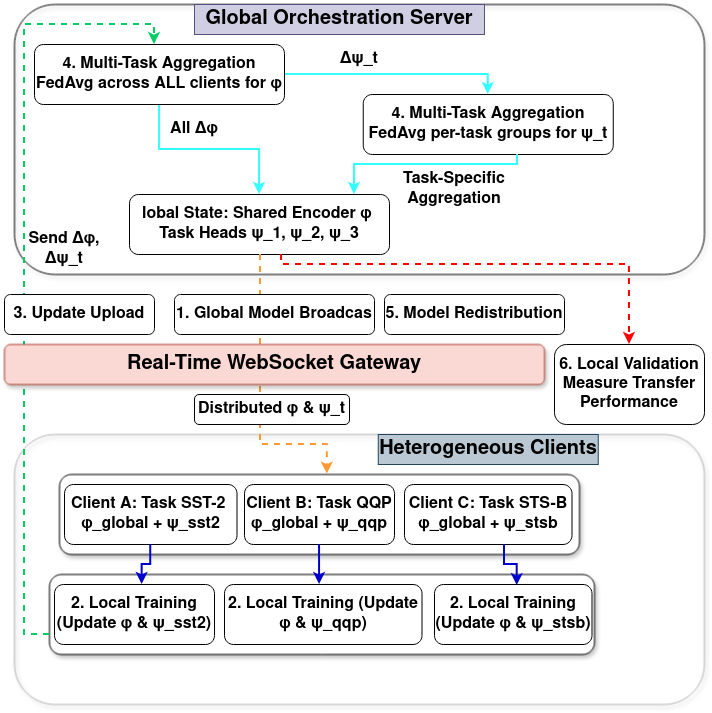
\includegraphics[width=1.0\textwidth]{plots/FL_MTL_FRAME_WORK.png}
    \caption{Architecture of the Proposed Real-time Federated Multi-Task Learning Framework. The system enables seamless integration of streaming data processing and collaborative model refinement.}
    \label{fig:framework_pipeline}
\end{figure*}

Federated components and privacy constraints of a system are based on:
\begin{itemize}
    \item Global server $\mathcal{S}$: coordinates client sampling, model broadcast, and aggregation.
    \item Distributed clients $\mathcal{C}$: edge devices/silos to store the raw text.
    \item Task set $\mathcal{K}$: the heterogeneous NLU tasks (intent classification, sentiment analysis, sequence labeling).
    \item Local datasets $\mathcal{D}_c^t$: single private, time-stamped data for client $c$ at round $t$ that is private.
\end{itemize}

Samples are never uploaded, for privacy purposes. Each client transmits only model updates (or compressed adapter and head updates) and serves as host-side aggregation \cite{mcmahan2017fedavg,elbakary2025mira}. This is consistent with the usual federated privacy model in which data locality is preserved and collaborative training is promoted in the field.

\subsection{Backbone of the Small Language Model}
This framework is adapted with specialized Small Language Models (SLMs) to trade-off computational efficiency and language fluency. Our current solution also supports DistilBERT \cite{sanh2019distilbert}, BERT-Medium \cite{devlin2018bert}, MiniLM \cite{wang2020minilm} architectures. These are shared feature extractors (encoder) that are fine-tuned collaboratively across the federated network. Our SLMs drastically minimize the communication overhead in contrast to standard-sized transformers.

\subsection{Multi-Task Learning Strategies}
We use a hybrid strategy of parameter-sharing. The lower layers of the transformer (encoder) are the same across the tasks that represent linguistic representation universally. In contrast, the top layers are task-specific classification or regression heads. We thus do an adaptive loss weighting mechanism to reduce the negative transfer:
\begin{equation}
    \mathcal{L}_{total} = \sum_{j=1}^{T} \alpha_j \mathcal{L}_j
\end{equation}
where $\alpha_j$ is dynamically tuned according to the convergence rate of each task $j$.

We define the parameters
\begin{equation}
\Theta = \{\theta_e, \{\theta_k\}_{k=1}^{K}\},
\end{equation}
for which $\theta_e$ is a common small-language-model encoder and $\theta_k$ is the task-based prediction head of task $k$ \cite{chen2024fedbone,zhou2025mfed,elbakary2025mira}. Prediction is for an input-output pair $(x,y)$ given task $k$.
\begin{equation}
\hat{y} = h_k\big(f_e(x;\theta_e);\theta_k\big),
\end{equation}
where $f_e(\cdot)$ represents the shared encoder and $h_k(\cdot)$ refers to the task head. It allows for parameter sharing amongst transferable linguistic traits but maintains task-level specialization.

\subsection{Federated Optimization and Real-time adaptation}
The process of federated optimization is detailed in Algorithm~\ref{alg:rt_fmtl}, which describes the federated optimization of the system. Clients will be able to update in real-time while the clients are still synchronizing updates asynchronously through WebSockets using this system to adapt in real-time. Updating the server aggregates updates with an example of a task-aware version of FedAvg (i.e. a version of FedAvg) and rounds off the updating with noise from heterogeneous data sources (Non-IID), but regularizes noise correctly.

\begin{algorithm}
\caption{RT-FMTL: Real-Time Federated Multi-Task Learning}
\label{alg:rt_fmtl}
\begin{algorithmic}[1]
\STATE \textbf{Server Initialize:} Shared core $\phi_0$, Task heads $\{\psi_{j,0}\}_{j=1}^T$
\FOR{each round $t = 1, 2, \dots$}
    \STATE Server transmits $\phi_t, \psi_{Task(k),t}$ to client $k \in K$ via WebSockets
    \FOR{each client $k \in K$ \textbf{in parallel}}
        \STATE Local training: $\{\Delta\phi_k, \Delta\psi_{Task(k),k}\} \leftarrow \text{LocalUpdate}(\mathcal{D}_k, \phi_t, \psi_{Task(k),t})$
        \STATE Updates $\{\Delta\phi_k, \Delta\psi_{Task(k),k}\}$ sent to Server using WebSockets
    \ENDFOR
    \STATE \textbf{Task-Aware Aggregation:}
    \STATE \quad $\phi_{t+1} \leftarrow \phi_t + \eta \sum_{k=1}^K \frac{n_k}{N} \Delta\phi_k$ \COMMENT{Universal Knowledge}
    \FOR{each task $j \in \{1,\dots,T\}$ \textbf{in parallel}}
        \STATE $\psi_{j,t+1} \leftarrow \psi_{j,t} + \eta \sum_{k \in K_j} \frac{n_k}{N_j} \Delta\psi_{j,k}$ \COMMENT{Heads Specialization}
    \ENDFOR
    \STATE Server redistributes $\{\phi_{t+1}, \psi_{Task(k),t+1}\}$ for Local Validation
\ENDFOR
\end{algorithmic}
\end{algorithm}

\subsection{Communication-Efficient Fine-Tuning (LoRA)}
To optimize resource utilization on edge devices even further, we implement Low-Rank Adaptation (LoRA) \cite{hu2021lora}. This includes when to update in local $B$, where instead of updating the full weight matrices $W \in \mathbb{R}^{d \times d}$, we optimize the low rank decomposition matrices $A$ and $B$, where:
\begin{equation}
W' = W + \Delta W = W + BA.
\end{equation}
$A \in \mathbb{R}^{r \times d}$ and $B \in \mathbb{R}^{d \times r}$ with rank $r \ll d$. For big updates, only the matrices $A$ and $B$ are sent, minimizing communication volume to up to 99\%.